\chapter{Despliegue} \label{cap:despligue}
\section{Entorno}
El entorno que se ha escogido para desplegar las partes del sistema que no residen en el dispositivo ubicuo ha sido Amazon Web Services (AWS). La razón es porque la empresa actualmente trabaja con este servicio y es más fácil integrarse con los módulos con los que se ha de integrar el sistema. AWS nos ofrece una serie de servicios que encajan con lo que se pretende desplegar.

El entorno que se ha escogido para desplegar las partes del sistema que residen en el dispositivo ubicuo ha sido Android. La razón es porque la empresa trabaja actualmente con dispositivos Android y tenía la necesidad de recolectar eventos en estos dispositivos.

\section{Máquinas}
El servicio que se ha escogido para desplegar las máquinas ha sido EC2\cite{Tfg:ec2}, ya que ofrece diferentes máquinas virtuales con diferentes características a nivel de hardware que pueden adaptarse notablemente a las necesidades de las diferentes partes del sistema.

\subsection{Subsistema de recolección y envío}
Para desplegar este subsistema tan solo se necesita un dispositivo Android. La versión mínima de Android ha de ser la 4.0 para que las librerías funcionen correctamente. El dispositivo ha de tener acceso a Internet para que pueda comunicarse con el subsistema de recepción e ingesta.

\subsection{Subsistema de recepción e ingesta}
\subsubsection{Módulo de recepción}
Este módulo hace un uso intensivo de CPU y red. Cuando a Kafka Rest Proxy se le hacen peticiones de POST, es decir, el módulo de envío no consume datos, explota el paralelismo de la CPU, a más cores, más peticiones podrá atender a la vez. El uso de RAM que hace este módulo es modesto y con que pueda soportar 1GB de heap es suficiente. El uso de red es elevado, puesto que ha de ser capaz de soportar diversas conexiones concurrentes en las cuales se pueden transmitir gran cantidad de datos. El uso de disco es mínimo, ya que no almacena ninguna información en ellos.
\\

La máquina escogida para desplegar este módulo ha sido la c5.2xlarge, en la tabla \ref{tabla:c5.2xlarge} se pueden ver sus recursos hardware.


\begin{table}[H]\label{tabla:c5.2xlarge}
	\centering
	\begin{tabular}{|l|l|}
		\hline
		\textbf{Máquina}            & \textbf{c5.2xlarge}    \\ \hline
		\textbf{CPUs}               & 8 cores                \\ \hline
		\textbf{RAM}                & 16.0 GiB               \\ \hline
		\textbf{Rendimiento de red} & Hasta 10 Gbps          \\ \hline
		\textbf{HDD tamaño}         & 30 GiB                 \\ \hline
		\textbf{HDD IOPS}           & X                      \\ \hline
	\end{tabular}
	\caption{Recursos hardware de la máquina virtual c5.2xlarge}
\end{table}



Para asegurar la confiabilidad del módulo y de paso aumentar el número de cores del sistema, se ha decidido desplegar 3 máquinas c5.2xlarge y un balanceador de carga que distribuya las conexiones entre las máquinas. Para desplegar el balanceador de carga se ha escogido utilizar el servicio que presta AWS de Aplication Load Balancer\cite{Tfg:apploadbalancer}.
\\
Con tal despliegue se puede soportar que caigan dos máquinas y aún el módulo podrá continuar haciendo su trabajo. Si ninguna máquina está caída se tendrán 24 cores y se podrán soportar conexiones de hasta 30 Gbps de tráfico agregado.

%%Foto

\subsubsection{Módulo de ingesta}
Este módulo hace un uso intensivo de RAM, red y disco. Para que Apache Kafka pueda funcionar necesita un orquestador que dirija y balancee los diferentes nodos (brokers) de Apache Kafka. Este orquestador es Apache Zookeeper. Apache Kafka y Apache Zookeeper hacen un uso diferente de los recursos, para no sobredimensionar las máquinas y reducir costes, Kafka y Zookeeper se desplegarán en máquinas con diferentes recursos.
\\\\
El uso que hace Kafka de los recursos es el siguiente:

\begin{itemize} 
	\item \textbf{CPU}: Hace un uso ligero de CPU, si se ha de elegir entre CPUs rápidas o con muchos cores, mejor una con muchos cores.
	\item \textbf{RAM}: Hace un uso intensivo de RAM, menos de 16 GB es improductivo.
	\item \textbf{Red}: Hace un uso intensivo de red, menos de 1 GbE es improductivo.
	\item \textbf{HDD}: Hace un uso intensivo de disco, se necesita espacio dependiendo del volumen de datos a tratar y un throughput elevado.
\end{itemize}

El uso que hace Zookeeper de los recursos es el siguiente:

\begin{itemize} 
	\item \textbf{CPU}: Hace un uso ligero de CPU.
	\item \textbf{RAM}: Hace un uso ligero de RAM, menos de 8 GB es improductivo.
	\item \textbf{Red}: Hace un uso intensivo de red, menos de 1 GbE es improductivo.
	\item \textbf{HDD}: Hace un uso intensivo de disco, se necesita un throughput elevado.
\end{itemize}

Con tales premisas, la máquina escogida para desplegar Apache Kafka ha sido la r4.xlarge, en la tabla \ref{tabla:kafkazookeeper} se pueden ver sus recursos hardware. La máquina escogida para desplegar Apache Zookeeper ha sido la r4.large, en la tabla \ref{tabla:c5.2xlarge} se pueden ver sus recursos hardware.

\begin{table}[H]\label{tabla:kafkazookeeper}
	\centering
	\begin{tabular}{|l|l|l|}
		\hline
		\textbf{Máquina}            & \textbf{r4.large} & \textbf{r4.xlarge} \\ \hline
		\textbf{CPUs}               & 2 cores           & 4 cores            \\ \hline
		\textbf{RAM}                & 15.25 GiB         & 30.5 GiB           \\ \hline
		\textbf{Rendimiento de red} & Hasta 10 Gbps     & Hasta 10 Gbps      \\ \hline
		\textbf{HDD tamaño}         & 30 GiB            & 500 GiB            \\ \hline
		\textbf{HDD IOPS}           & X                 &  X                 \\ \hline
	\end{tabular}
	\caption{Recursos hardware de la máquina virtual r4.large y r4.xlarge}
\end{table}

Zookeeper necesita un mínimo de 3 máquinas para funcionar, por lo que se han desplegado 3 máquinas r4.large.
Kafka no tiene un número mínimo de máquinas para funcionar, pero para aumentar la confiabilidad, la durabilidad y el rendimiento, se han desplegado 3 máquinas r4.xlarge.

\subsection{Subsistema de transformación}
El despliegue del subsistema de transformación es particular puesto que un módulo ya está desplegado en la empresa. Para dar completud al trabajo, en aquellos módulos que ya estén desplegados, se hablará de las máquinas que se desplegarán para hacer la demostración el día de la lectura del trabajo.

\subsubsection{Módulo de transformación}
Al estar dividido el módulo de transformación en dos submódulos y encargarse de tareas diferentes, el uso de los recursos es diferente en los dos submódulos. 
\\
Para el submódulo de propósito específico se ha desplegar Logstash, en la documentación de la herramienta no se deja del todo claro los requerimientos hardware, pero por su naturaleza se ha supuesto que hace un uso intensivo de CPU, RAM y red, y un uso ligero de disco. De momento se ha desplegado en una r4.xlarge, en la tabla \ref{tabla:kafkazookeeper} se puede ver sus recursos hardware. Como trabajo futuro, se ha monitorear el rendimiento de este submódulo para ver el uso de los recursos que hace, y cambiar si fuera necesario la máquina utilizada.
\\
Para el submódulo de propósito general se ha de desplegar la aplicación Java que utiliza Kafka Streams. El despliegue de máquinas para este submódulo depende mucho del volumen de datos que se hayan de procesar, para la demostración se va a suponer un volumen de datos pequeño, tan solo para verificar que la solución funciona. La máquina escogida es una t2.micro en la tabla \ref{tabla:t2.micro} se pueden ver sus recursos hardware.

\begin{table}[H]\label{tabla:t2.micro}
	\centering
	\begin{tabular}{|l|l|}
		\hline
		\textbf{Máquina}            & \textbf{t2.micro}      \\ \hline
		\textbf{CPUs}               & 1 cores                \\ \hline
		\textbf{RAM}                & 1.0 GiB                \\ \hline
		\textbf{Rendimiento de red} & Moderado               \\ \hline
		\textbf{HDD tamaño}         & 30 GiB                 \\ \hline
		\textbf{HDD IOPS}           & X                      \\ \hline
	\end{tabular}
	\caption{Recursos hardware de la máquina virtual t2.micro}
\end{table}

Se van a desplegar 3 máquinas r4.xlarge para el submódulo de propósito específico, con el objetivo de distribuir la carga entre los servidores y aumentar la potencia de procesado.
\\
Se va a desplegar 1 máquina t2.micro para el submódulo de propósito general, con el objetivo de comprobar la solución propuesta.

\subsection{Módulo de almacenamiento}
Este módulo ya está desplegado en la empresa, por lo que el despliegue que se ha hecho es exclusivo para la demostración. Por un lado se ha desplegado un cluster de Elastic Search y una máquina con Kibana, y por otro una máquina con JIRA.

Para el despliegue del cluster de Elastic Search se han utilizado máquinas parecidas a las que utiliza la empresa. La máquina escogida es una r4.xlarge, en la tabla \ref{tabla:kafkazookeeper} se puede ver sus recursos hardware. Para el despligue de Kibana se ha utilizado una t2.micro, ya que JIRA no consume grandes recursos, en la tabla \ref{tabla:t2.micro} se puede ver los recursos hardware de la máquina escogida.
\\
Para el despligue de JIRA se va a utilizar una t2.small ya que JIRA como mínimo requiere 2 GiB de RAM para funcionar fluido. En la tabla \ref{tabla:t2.small} se puede ver los recursos hardware de la máquina escogida.

\begin{table}[H]\label{tabla:t2.small}
	\centering
	\begin{tabular}{|l|l|}
		\hline
		\textbf{Máquina}            & \textbf{t2.small}      \\ \hline
		\textbf{CPUs}               & 1 cores                \\ \hline
		\textbf{RAM}                & 2.0 GiB                \\ \hline
		\textbf{Rendimiento de red} & Moderado               \\ \hline
		\textbf{HDD tamaño}         & 30 GiB                 \\ \hline
		\textbf{HDD IOPS}           & X                      \\ \hline
	\end{tabular}
	\caption{Recursos hardware de la máquina virtual t2.small}
\end{table}

Se van a desplegar 3 máquinas r4.xlarge para Elastic Search ya que se quiere comprobar el correcto funcionamiento del sistema cuando Elastic Search está distribuido en más de una máquina. Se va desplegar 1 máquina t2.micro para Kibana. Se va a desplegar una máquina t2.small para JIRA.

\subsection{Resumen de servicios a desplegar}

\begin{table}[H]\label{tabla:resumenservicios}
	\centering
	\resizebox{15cm}{!}{
	\begin{tabular}{|l|l|l|l|l|}
		\hline
		\textbf{Módulo} & \textbf{Aplicación} & \textbf{Servicio}      & \textbf{Detalle}          & \textbf{Número} \\ \hline
		Recepción       & Kafka Rest Proxy    & Amazon EC2             & c5.2xlarge                & 3               \\ \hline
		Recepción       & Kafka Rest Proxy    & Elastic Load Balancing & Application Load Balancer & 1               \\ \hline
		Ingesta         & Apache Kafka        & Amazon EC2             & r4.xlarge                 & 3               \\ \hline
		Ingesta         & Apache Zookeeper    & Amazon EC2             & r4.large                  & 3               \\ \hline
		Transformación  & Logstash            & Amazon EC2             & r4.xlarge                 & 3               \\ \hline
		Transformación  & Kafka Streams       & Amazon EC2             & t2.micro                  & 1               \\ \hline
		Almacenamiento  & Elastic Search      & Amazon EC2             & r4.xlarge                 & 3               \\ \hline
		Almacenamiento  & Kibana              & Amazon EC2             & t2.micro                  & 1               \\ \hline
		Almacenamiento  & JIRA                & Amazon EC2             & t2.small                  & 1               \\ \hline
	\end{tabular}
    }
	\caption{Recursos de servicios a desplegar}
\end{table}

En la tabla \ref{tabla:resumenservicios} se pueden ver el resumen de los servicios a desplegar en AWS. La columna \textit{Módulo} nos dice el módulo del sistema que se despliega, la columna \textit{Aplicación} nos marca la aplicación que se va a desplegar, la columna \textit{Servicio} no dice el servicio de AWS que se va a utilizar, la columna \textit{Detalle} nos informa sobre que servicio en concreto se va a desplegar y la columna \textit{Número} no dice el número de instancias que se van a desplegar. Cada fila corresponde a los servicios a desplegar.

\subsection{Networking}

\begin{figure}[!htb]
	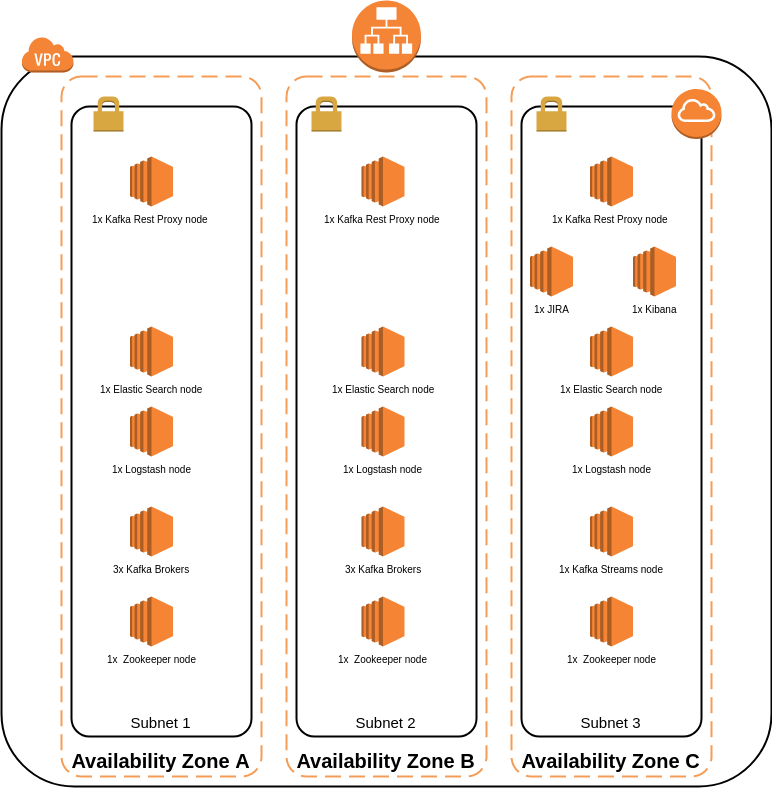
\includegraphics[width=\linewidth] {Moduloss-netdeploy.png}
	\caption{Networking del despliegue en AWS}
	\label{fig:networking1}
\end{figure}

En la figura \ref{fig:networking1} se puede ver el como queda el despliegue de red de las máquinas, en el anexo X se explica la leyenda de los iconos. Para interconectar las diferentes máquinas, AWS son ofrece el servicio Amazon Virtual Private Cloud (Amazon VPC), esta VPC es una red virtual que interconecta las máquinas virtuales que se han desplegado, funciona igual que una red local tradicional. En la figura \ref{fig:networking1} se puede ver como existen 3 subredes que residen en 3 Availability Zones diferentes. AWS trabaja con los conceptos de región y zonas de disponibilidad. La VPC reside en una región, una región es una porción geográfica de un país. Las zonas de disponibilidad son diferentes data centers dentro de la región. En el caso de la figura, el sistema reside en una zona y está disperso entre los diferentes data centers de la zona. Se ha hecho así para aumentar la confiabilidad del sistema ya que tal y como se han configurado los diferentes módulos, el sistema es tolerante a caídas de servidores, y desplegarlos en diferentes zonas de disponibilidad disminuye la posibilidad de que caigan dos máquinas a la vez del mismo módulo.
\\\\
La figura \ref{fig:networking1} también muestra que la VPC está encabezada por un Aplication Load Balancer, este balanceador de carga es el que recibe las peticiones del dispositivo ubicuo y distribuye la carga entre los 3 Kafka Rest Proxy nodes. Por último, la figura muestra en la Subnet 3 una Internet Gateway, se ha añadido para que las máquinas de JIRA y de Kibana sean accesibles desde Internet.


